\documentclass{article}%
\usepackage[T1]{fontenc}%
\usepackage[utf8]{inputenc}%
\usepackage{lmodern}%
\usepackage{textcomp}%
\usepackage{lastpage}%
\usepackage{geometry}%
\usepackage{setspace}%
\usepackage{booktabs}%
\usepackage{float}%
\usepackage{graphicx}%
\usepackage{pgfgantt}%
\usepackage{fancyhdr}%
\usepackage[hidelinks]{hyperref}%
%
\renewcommand{\contentsname}{Summary}%
\pagestyle{fancy}%
\setlength{\headwidth}{510pt}%
\fancyhead[L]{
\includegraphics[width=2cm]{frigel-logo.png}}%
\fancyhead[C]{\textbf{Project Proposal}}%
\fancyhead[R]{
\includegraphics[width=1cm]{unifi-logo.png}}%
\setlength{\headheight}{2cm}%
%
\begin{document}%
\normalsize%
\newgeometry{top=1cm, bottom=2cm, left=2cm, right=2cm}%
\begin{titlepage}%
\centering%
\vspace*{1cm}%

    \begin{minipage}{0.45\textwidth}
    
\includegraphics[scale=0.5]{frigel-logo.png}
    \end{minipage}
    \hfill
    \begin{minipage}{0.45\textwidth}
    \begin{flushright}
        
\includegraphics[scale=0.1]{unifi-logo.png}
    \end{flushright}
    \end{minipage}
    \\[1.5cm]
    %
\Huge\textbf{Project Proposal}\\[0.5cm]%
\Large\textbf{Automatic Manual Development}\\[2cm]%
\large Romeo Bandinelli, Djonathan Quadras\\%
\large Università degli Studi di Firenze\\[2cm]%
\large April, 2025%
\vfill%
\end{titlepage}%
\newgeometry{top=3.5cm, bottom=2cm, left=2cm, right=2cm}%
\onehalfspacing%
\setlength{\parindent}{12pt}%
\tableofcontents%
\newpage%
\section{About the Project}%
\label{sec:AbouttheProject}%
Fashion for Future, a research lab at the University of Florence, proposes a project to Frigel, a leading manufacturer of cooling and temperature control machines.  This initiative focuses on automating the currently manual development process for new machine releases, significantly improving efficiency and reducing development time.  The project will leverage advanced technologies to streamline workflows and optimize the entire production lifecycle.

%
\subsection{About the Team}%
\label{subsec:AbouttheTeam}%
The Fashion For Future research lab is a multidisciplinary and multi-skilled environment focused on bridging the gap between academia and industry by connecting technological development with practical application. Within this framework, various projects are organized to empower professionals in the use of artificial intelligence tools.  \\ 
The technical and scientific lead is Prof. Dr. Romeo Bandinelli, Associate Professor in the Department of Industrial Engineering at the University of Florence (Italy) with expertise on management and innovation of industrial processes, with a special focus on the dynamics of product lifecycle management and supply chain operations. He is also a co-founder of Balance, a start-up that supports companies in production planning and continuous improvement initiatives. \\ 
The team also includes the researcher Djonathan Luiz de Oliveira Quadras. He has worked on projects involving databases integration, development of managerial dashboards using BI tools, and the application of machine learning and AI for automated data analysis and reporting. His current doctoral project focuses on applying AI to fashion supply chains, with an emphasis on data-driven decision-making support for businesses. \\ 

%
\newpage%
\section{Proposed Solution}%
\label{sec:ProposedSolution}%
This section proposes an automated solution for generating technical manuals, significantly reducing the time and resources currently required for manual creation.  This automated approach offers improved consistency, scalability, and the potential for multilingual support, ultimately streamlining the entire manual production process.\newline%
The figure below illustrates the proposed framework.  The process begins with data collection from various internal company sources. This diverse data is then structured and consolidated within a central database, serving as the system's primary data source.  This unified dataset is subsequently fed into machine learning algorithms to cluster similar machines and identify their key properties based on data from existing machines.  Finally, these clustered data points and classifications are utilized by large language models to generate human{-}readable descriptions in multiple languages, resulting in the automatic generation and export of complete manuals in the desired format.%


\begin{figure}[h!]%
\centering%
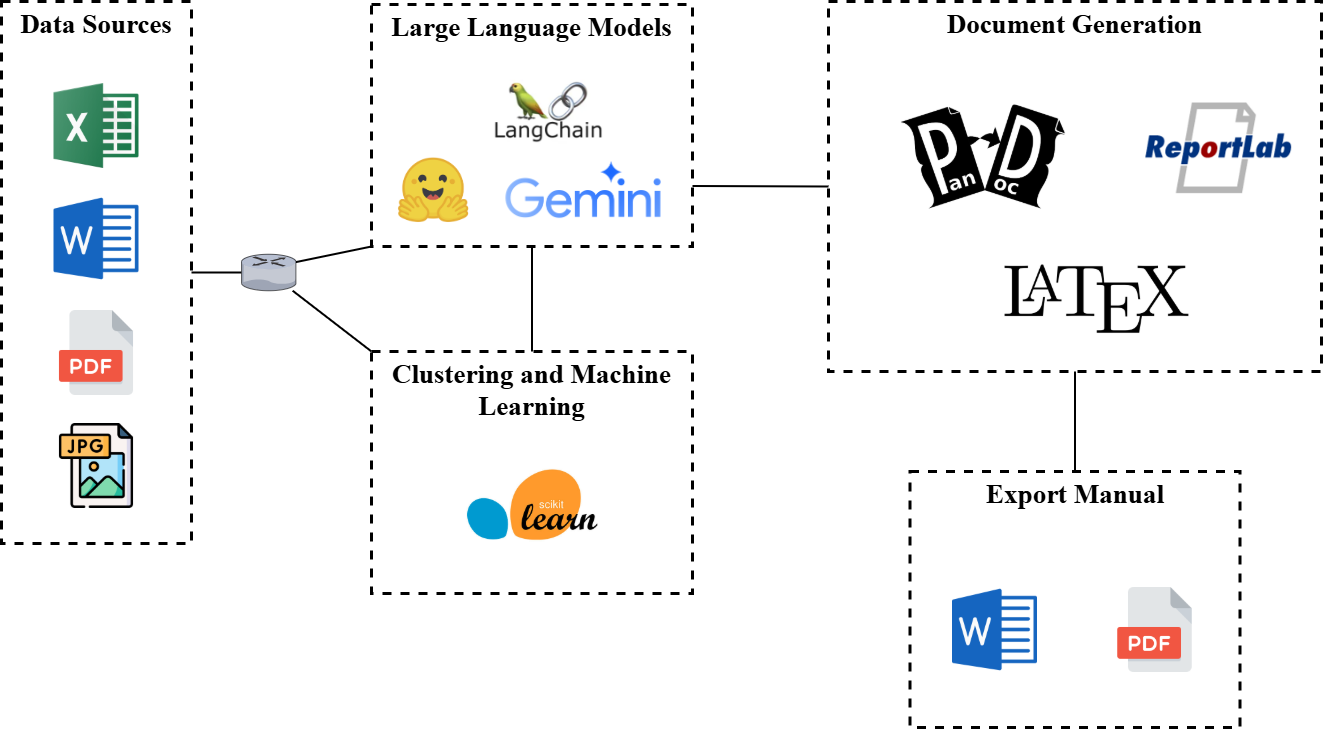
\includegraphics[width=0.8\textwidth]{images/Tools.png}%
\caption{Proposed Framework.}%
\end{figure}

%
\subsection{Data Sources}%
\label{subsec:DataSources}%
Developing comprehensive manuals for cooling machines necessitates a multi{-}source data gathering process.  Information is drawn from various sources including the company's Enterprise Resource Planning (ERP) system, engineering team{-}provided Excel spreadsheets, descriptive Word documents, and PDFs containing specifications and diagrams from previous models.\newline%
This diverse data compilation ensures the manual's accuracy and completeness, encompassing both technical specifications and operational details.  The integration of data from disparate formats requires careful organization and verification to produce a user{-}friendly and reliable document.

%
\subsection{Large Language Models}%
\label{subsec:LargeLanguageModels}%
Large Language Models (LLMs) can significantly automate machine manual generation by processing technical specifications and transforming them into user{-}friendly documentation.  LLMs can understand complex technical jargon and translate it into plain language, generate different versions tailored to various user skill levels, and even incorporate images and diagrams based on provided data.  This automation can be achieved using Python packages like Langchain, Hugging Face's Transformers, and Google's Gemini, which provide the necessary tools for interacting with and fine{-}tuning LLMs for this specific task.\newline%
Langchain offers tools to orchestrate the LLM workflow, connecting it to external data sources like databases containing machine specifications. Hugging Face provides access to a wide range of pre{-}trained LLMs and tools for fine{-}tuning them on specific datasets of machine documentation to improve accuracy and style.  Gemini, a powerful LLM, can directly generate and structure the manual text, potentially integrating multimedia elements.  These packages work together or independently to create a complete pipeline for automatic machine manual generation, from data ingestion and processing to final document creation.

%
\subsection{Clustering and Machine Learning}%
\label{subsec:ClusteringandMachineLearning}%
Clustering in machine learning is an unsupervised learning technique that groups similar data points together into clusters.  The goal is to find inherent structure in the data without pre{-}defined labels.  In the context of cooling and temperature control machines, clustering could analyze data like energy consumption, operational parameters (temperature settings, run times, etc.), maintenance history, and error logs.  By clustering these machines based on their feature similarities, one could identify groups of machines with similar performance characteristics, potentially revealing patterns in machine efficiency, failure modes, or optimal operating conditions. This allows for more targeted maintenance, optimized resource allocation, and improved system{-}wide performance analysis.\newline%
Scikit{-}learn (sklearn) is a popular Python library for machine learning that provides various algorithms for data mining and data analysis.  For clustering machines based on their characteristics, several algorithms within Scikit{-}learn could be applied.  These include K{-}Means clustering (for partitioning data into k clusters), hierarchical clustering (building a hierarchy of clusters), DBSCAN (Density{-}Based Spatial Clustering of Applications with Noise, for identifying clusters of arbitrary shape), and Gaussian Mixture Models (assuming data points are generated from a mixture of Gaussian distributions).  The choice of algorithm depends on the specific characteristics of the data and the desired outcome of the clustering analysis.

%
\subsection{Document Generation}%
\label{subsec:DocumentGeneration}%
Generating documents in a specific format and template using Python involves leveraging libraries that handle document structure and formatting.  These libraries allow for programmatic creation of documents by defining content, styles, and layouts within the code, ultimately producing output files such as PDFs or Word documents that adhere to the desired template. For this purpose, packages like Pylatex, ReportLab, and Pandoc can be used.\newline%
Pylatex allows for the generation of LaTeX documents, providing control over the formatting through LaTeX commands embedded within Python code. ReportLab offers a more Pythonic approach, enabling the creation of PDFs directly from Python scripts using a drawing{-}based model.  Pandoc acts as a universal document converter, allowing conversion between various formats like Markdown, LaTeX, and DOCX.  By using Pandoc in conjunction with a templating engine, a Python script could generate a document in a specified format and then leverage Pandoc's conversion capabilities to output the desired file type according to a pre{-}defined template.

%
\newpage%
\section{Timetable and Activities}%
\label{sec:TimetableandActivities}%

        "This section presents the timetable and task descriptions for the
        project development. The project is structured into six main steps,
        with two intermediate milestones. The total estimated duration is
        sixteen weeks, and the involvement of at least two researchers is
        required..
        %
\begin{figure}[htbp]%
\centering%

        \begin{ganttchart}{0}{17}
        \gantttitle{Project Planning in Weeks}{18} \\
        \gantttitlelist{0,...,17}{1} \\
        \ganttgroup{Project}{1}{16} \\
        \ganttbar{Data Collection}{1}{4} \\
        \ganttmilestone{Process Map}{4} \ganttnewline
        \ganttlinkedbar{Machine Learning Modelling}{5}{8} \ganttnewline
        \ganttlinkedbar{Prompt Modelling for LLM}{9}{10} \ganttnewline
        \ganttlinkedbar{Template Development}{5}{12} \ganttnewline
        \ganttlinkedbar{Validation}{13}{14} \ganttnewline
        \ganttmilestone{Automated process}{14} \ganttnewline
        \ganttlinkedbar{Training}{15}{16} \ganttnewline
        \ganttmilestone{Project Finish}{16}
        \ganttlink{elem1}{elem2}
        \ganttlink{elem2}{elem3}
        \ganttlink{elem2}{elem5}
        \ganttlink{elem6}{elem7}
        \ganttlink{elem7}{elem8}
        \ganttlink{elem8}{elem9}
        
        \end{ganttchart}

        %
\end{figure}%
\subsection{Data Collection}%
\label{subsec:DataCollection}%
The Data Collection phase will involve conducting interviews with relevant departments and manual developers.  This will map the entire process, identify all components and stakeholders, define quality criteria, and gather necessary data for subsequent project phases.  The deliverable for this phase, representing the first project milestone, is a comprehensive process map. This phase is estimated to require a minimum of four weeks.

%
\subsection{Machine Learning Modelling}%
\label{subsec:MachineLearningModelling}%
The Machine Learning Modelling section encompasses data analysis of the previously collected dataset, followed by the application and fitting of machine learning algorithms to cluster machines and identify similarities.  This crucial step, requiring a minimum of four weeks, provides the foundation for subsequent project phases.  Its outputs—the resulting machine clusters and similarity analysis—are essential for accurate machine descriptions and information completion in the final report.

%
\subsection{Prompt Modelling for LLM}%
\label{subsec:PromptModellingforLLM}%
Prompt modeling for the Large Language Model (LLM) will involve defining optimal prompts for each section of the manual. This process aims to identify the most effective prompting strategies and text inputs to generate accurate and consistent outputs aligned with the manual's requirements.  The goal is to minimize inaccuracies and ensure textual coherence. This phase is allocated a minimum of two weeks.

%
\subsection{Template Development}%
\label{subsec:TemplateDevelopment}%
The Template Development phase will encompass the design and creation of LaTeX and PyLaTeX templates for manual generation.  This is crucial for ensuring consistent quality and a standardized format across all manuals.  Automated generation via these templates will streamline the process. This phase is estimated to require a minimum of nine weeks.

%
\subsection{Validation and Training}%
\label{subsec:ValidationandTraining}%
The project includes a two{-}week validation phase, conducted collaboratively with a company intern, to assess the generated manual's quality and implement necessary revisions.  Following validation, a four{-}week training program will be delivered to the manual development department. This training will cover the developed solution's functionality, operation, and the revised process implementation, encompassing two weeks of theoretical instruction and two weeks of practical application.

%
\newpage%
\section{Final Considerations}%
\label{sec:FinalConsiderations}%
The proposed project has the potential to significantly enhance both the efficiency and speed of manual development processes. Currently, these processes involve several time-consuming manual tasks that do not add value to the final product. Technicians often spend considerable time adjusting templates and aggregating information — activities that could be easily handled by software. Also, existing Generative AI platforms and APIs are already capable of structuring ideas, correcting grammar, and improving the overall coherence of texts.

As a simple demonstration of the model’s effectiveness, this entire document was developed using it. The template was generated by combining Python and LaTeX code. The figure below shows the working environment of this project. You can find the repository with all codes \href{ https://github.com/djonquadras/ManualDevelopment}{here.}

\begin{figure}[H]
\centering
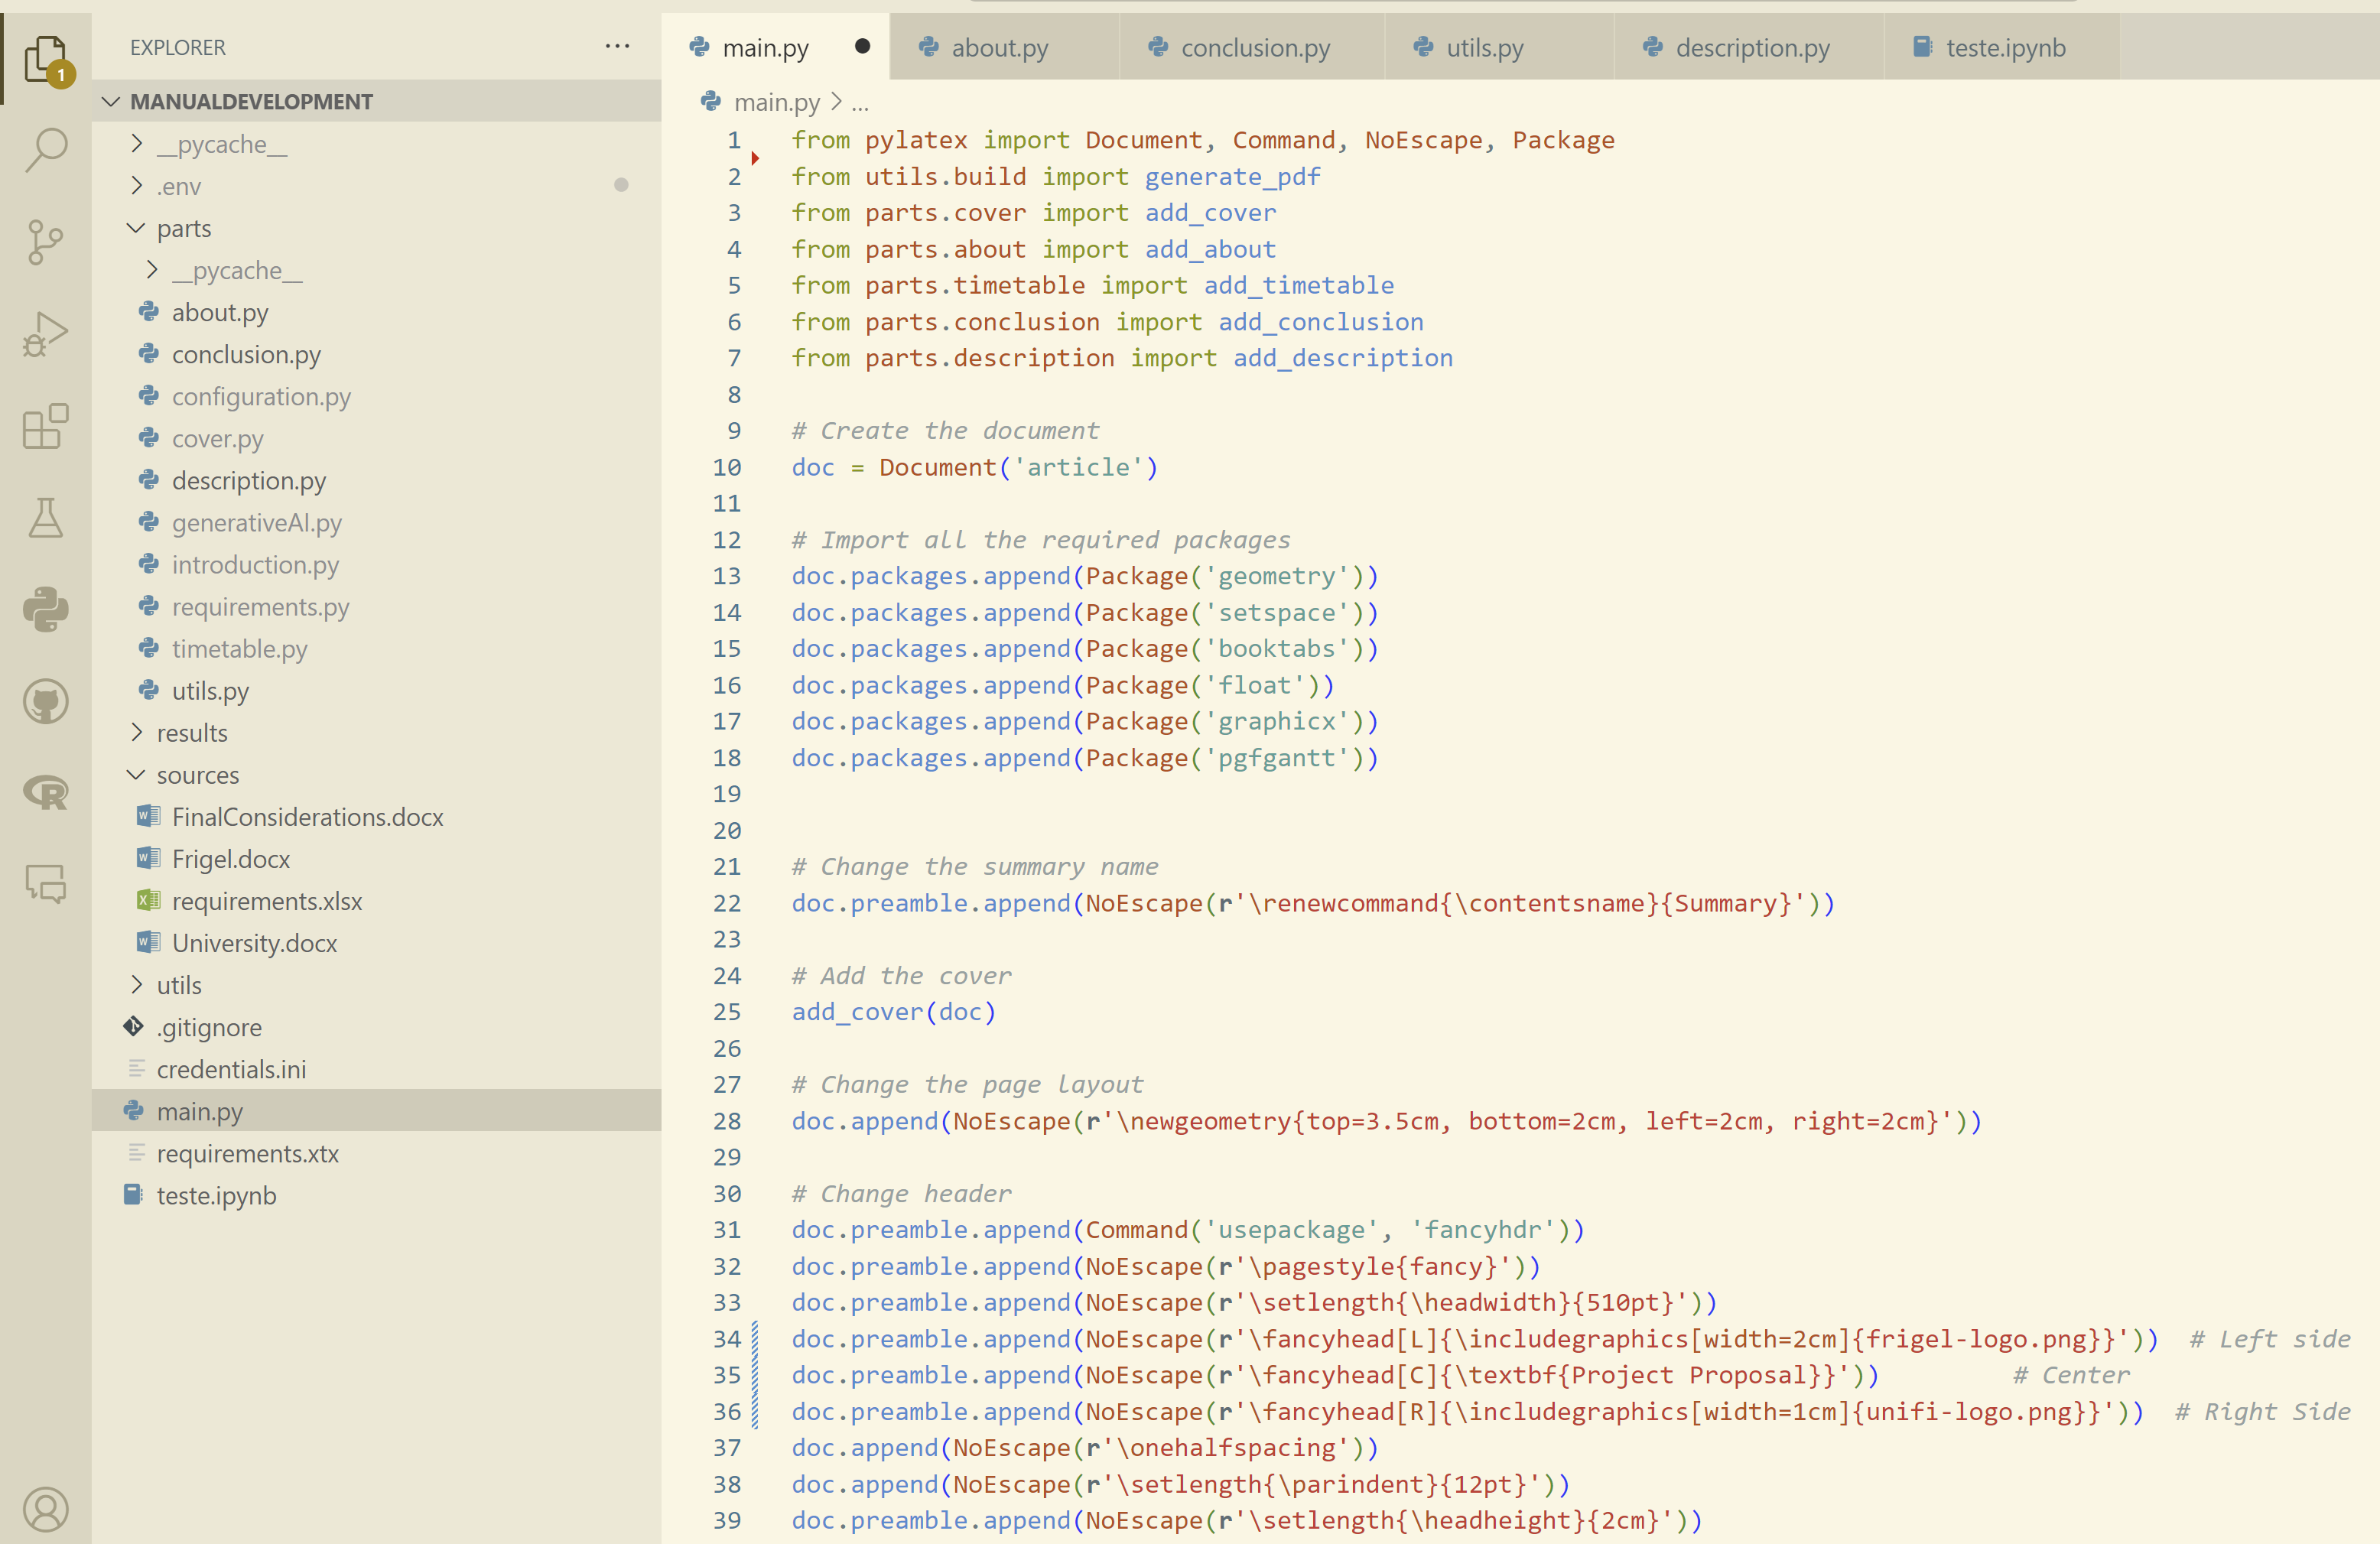
\includegraphics[width=0.8\textwidth]{images/doc1/image1.png}
\end{figure}

The “About the Project” section was developed by a mix of GenAI (using Gemini API) and personal texts.

\begin{figure}[H]
\centering
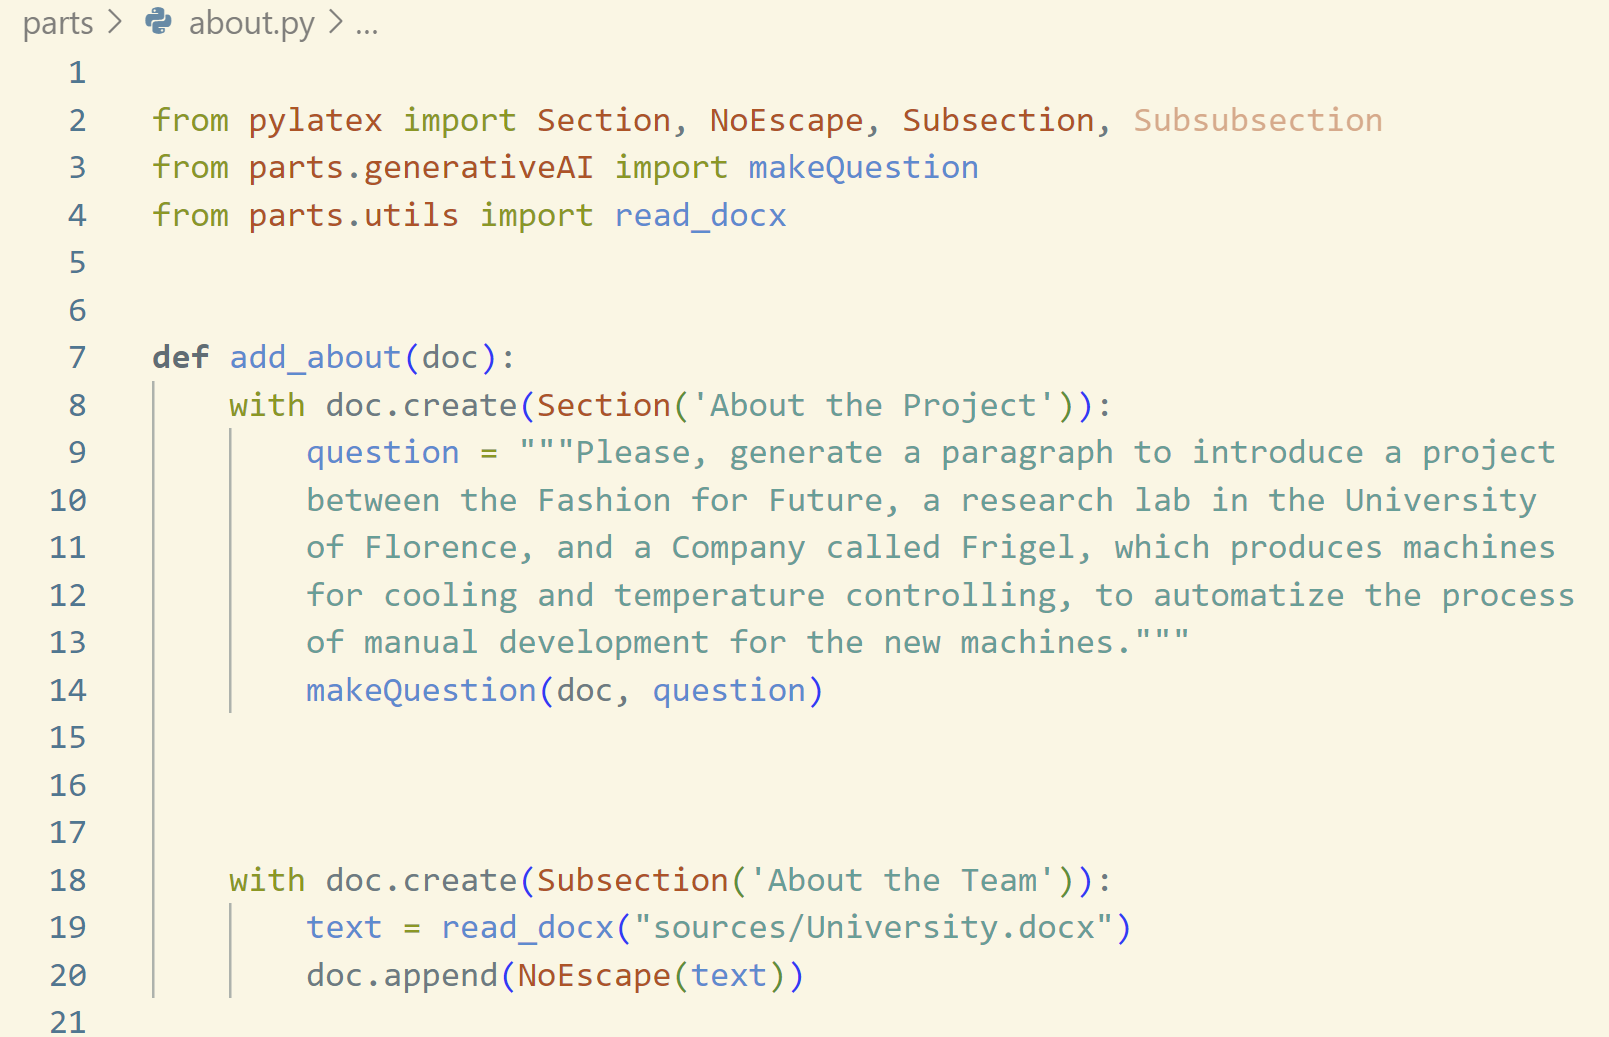
\includegraphics[width=0.8\textwidth]{images/doc1/image2.png}
\end{figure}

On the other hands, for the “Proposed Solution” section, besides the image that was fully developed manually, all the texts were generated by GenAI.

\begin{figure}[H]
\centering
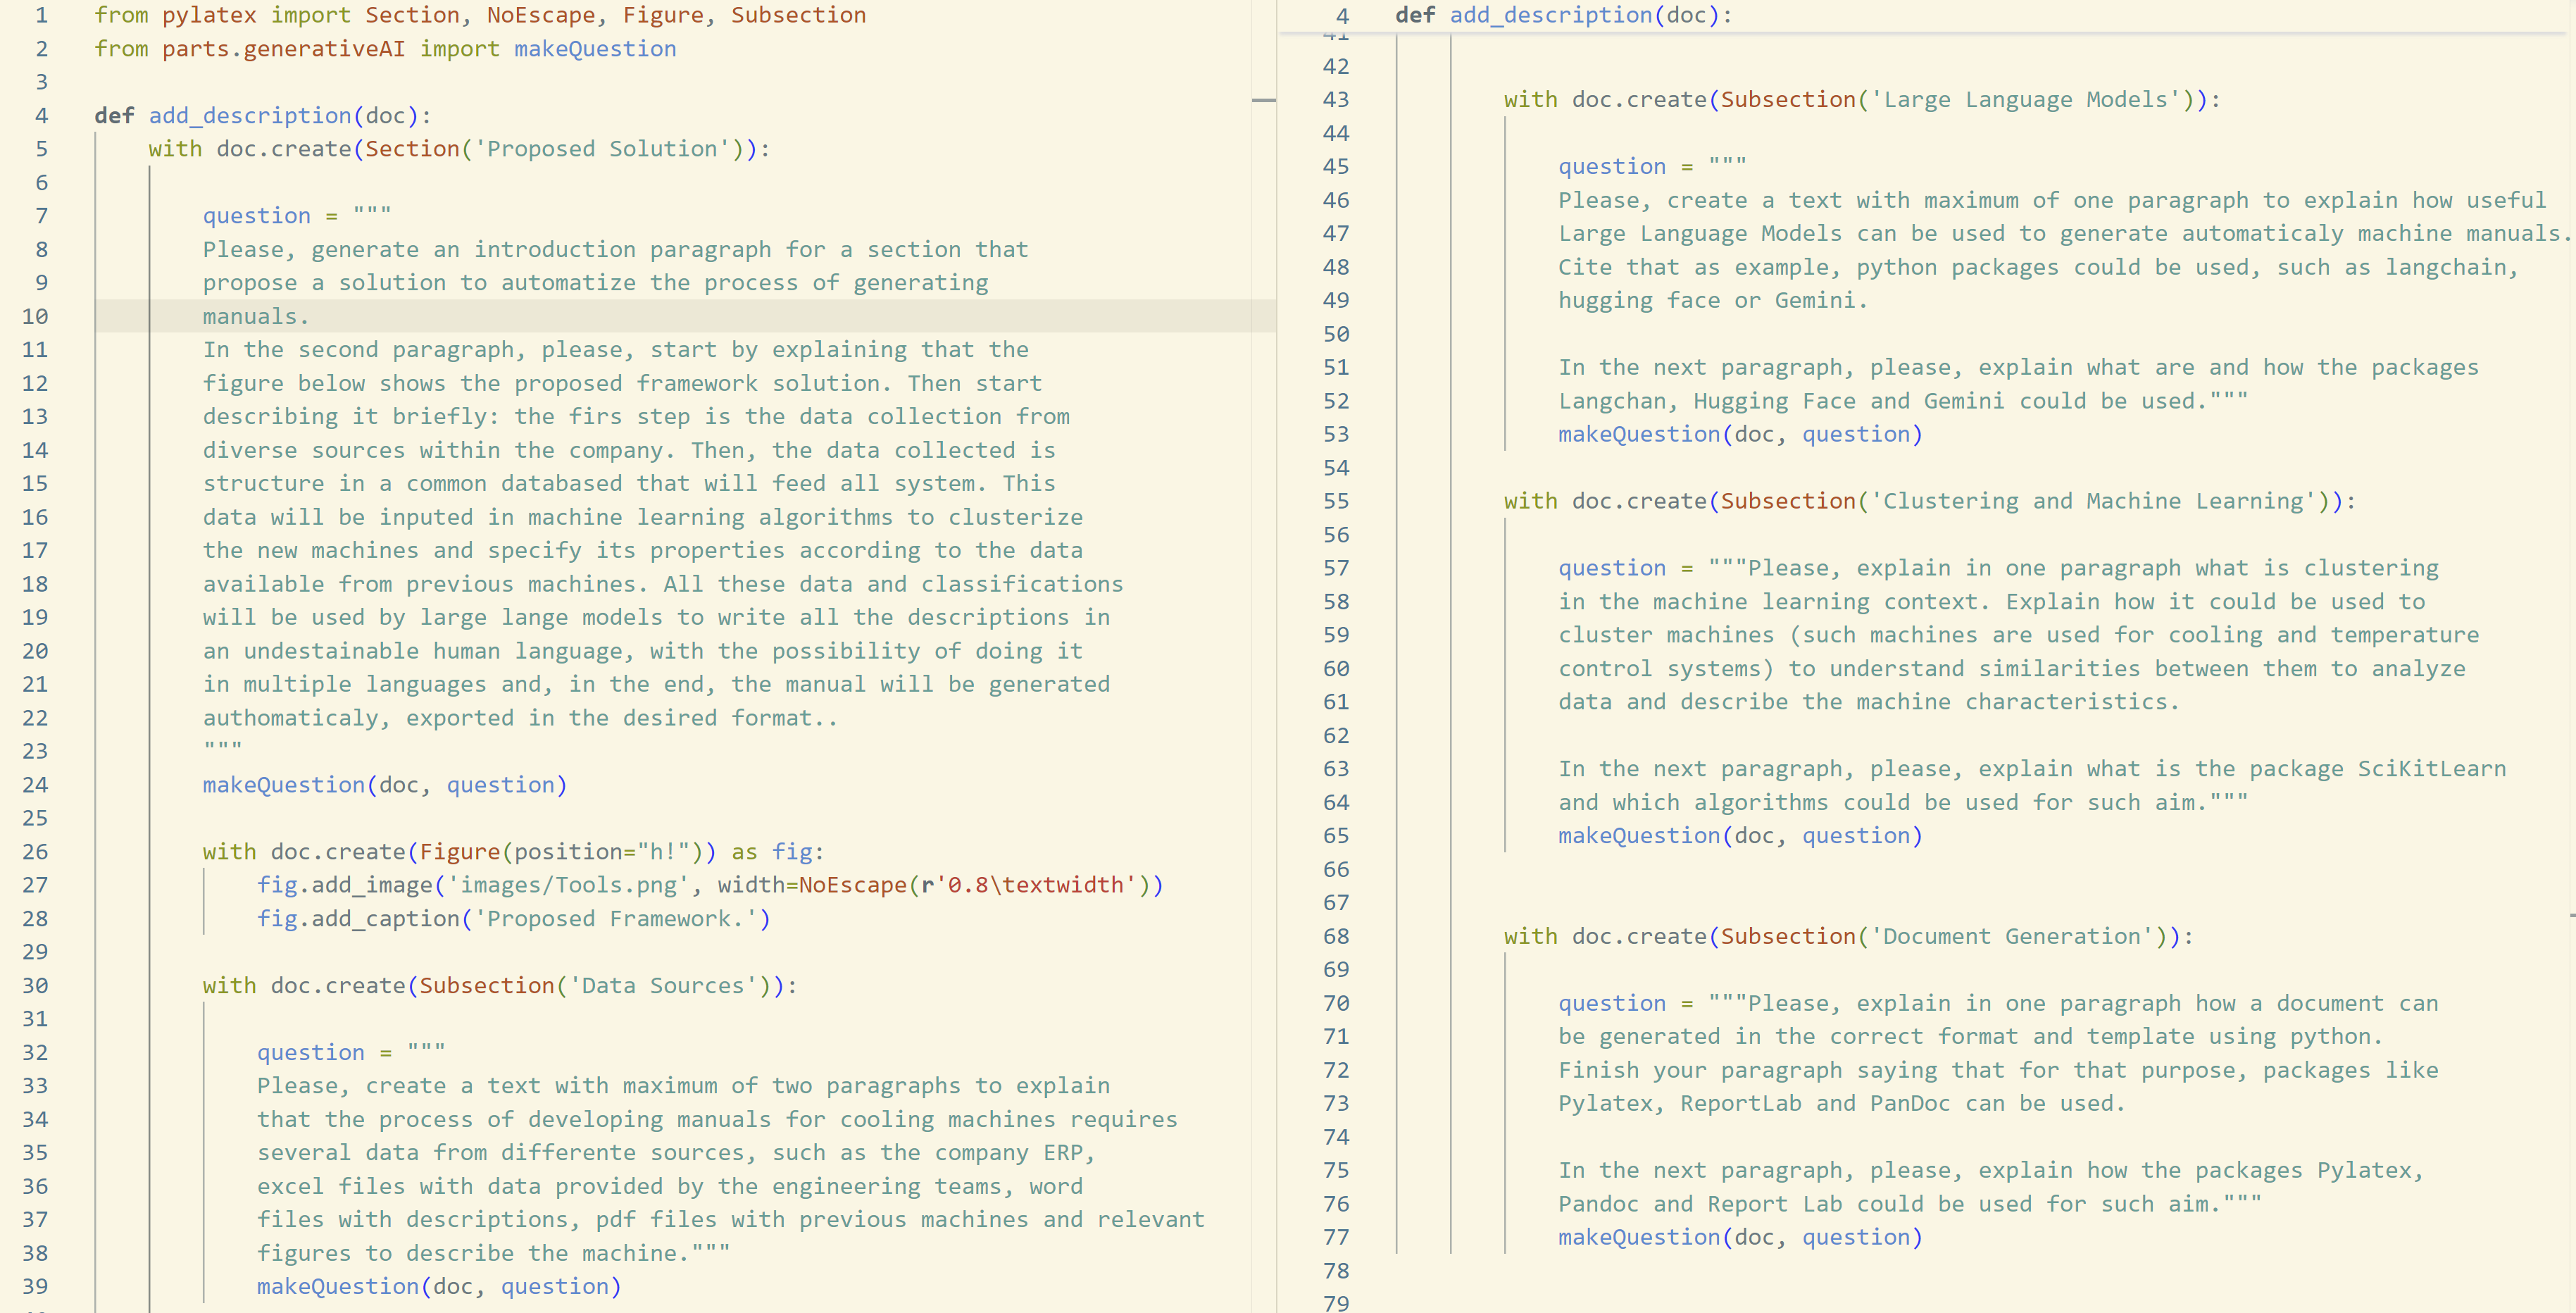
\includegraphics[width=0.8\textwidth]{images/doc1/image3.png}
\end{figure}

Finally, this conclusion section was fully written in a word file, with the figures placed in the desired positions, and the code successfully collected all the information and placed in the desired positions.

\begin{figure}[H]
\centering
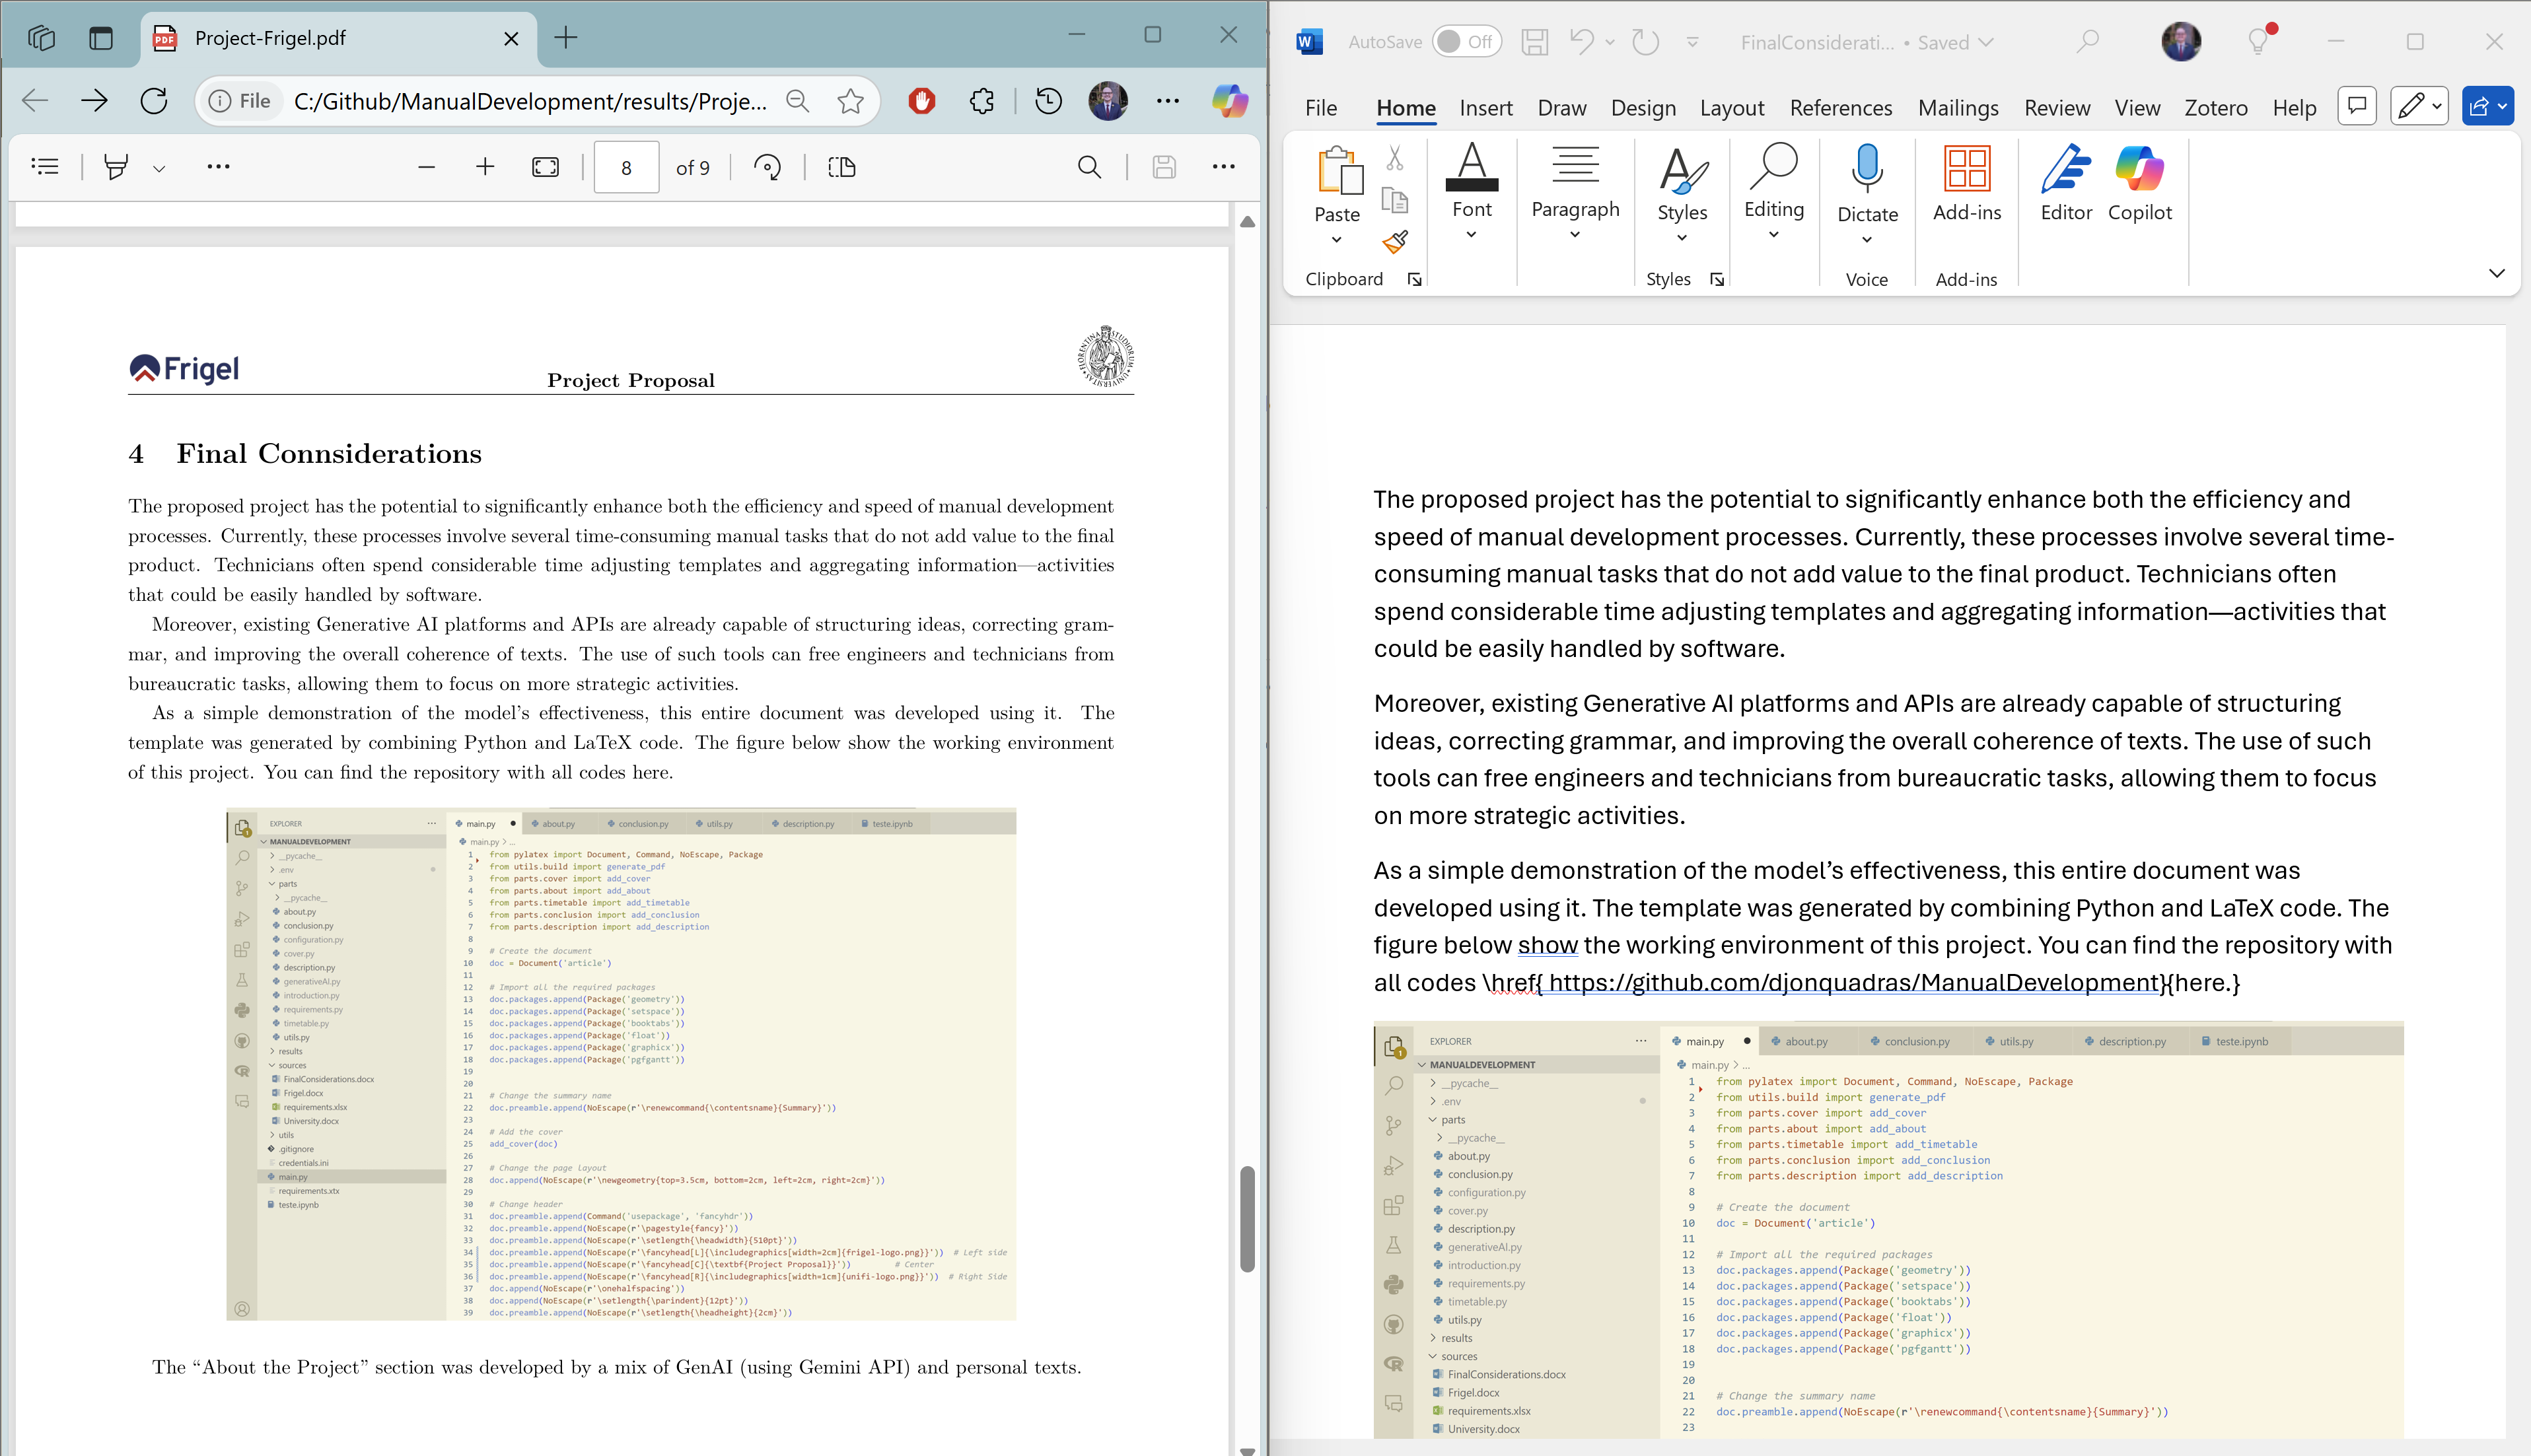
\includegraphics[width=0.8\textwidth]{images/doc1/image4.png}
\end{figure}

This simple example demonstrates that the proposed framework is a feasible solution to support the manual development team in enhancing work efficiency, enabling the delivery of manuals in a faster, simpler, and smarter way.

%
\end{document}